\documentclass[12pt]{article}

\title{Is Florida getting warmer}

\usepackage{graphicx}
%\usepackage{subfig}
\usepackage{caption}
\usepackage{subcaption}

\begin{document}
    \maketitle

    \section{Introduction}
        This report checks whether Florida is getting warmer over the years. It checks whether the correlation between the variables is a result of chance or if it is significant by itself

    \section{Methods}
        The correlation between the temperature and year is calculated using the cor function in R. 
        The significance of this observed correlation is verified using the a permutation analysis. 

    \section{Results}    
    \begin{figure}
        \centering
        \begin{subfigure}{.5\textwidth}
          \centering
          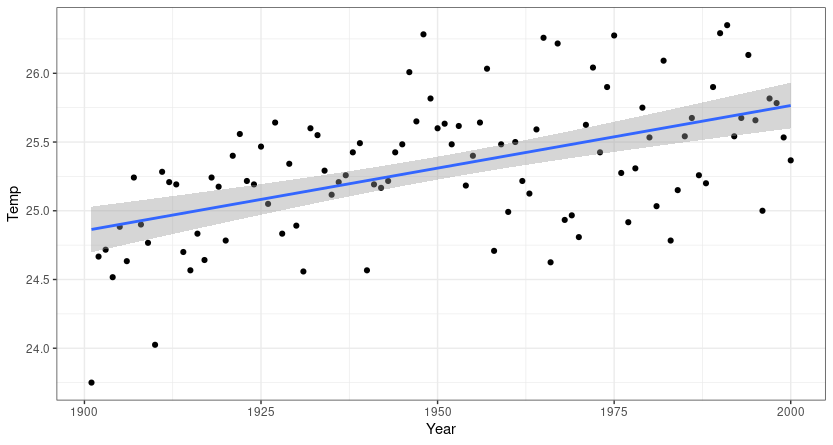
\includegraphics[width=.75\linewidth]{../../week3/data/latex1.png}
          \caption{A subfigure}
          \label{fig:sub1}
        \end{subfigure}%
        \begin{subfigure}{.5\textwidth}
          \centering
          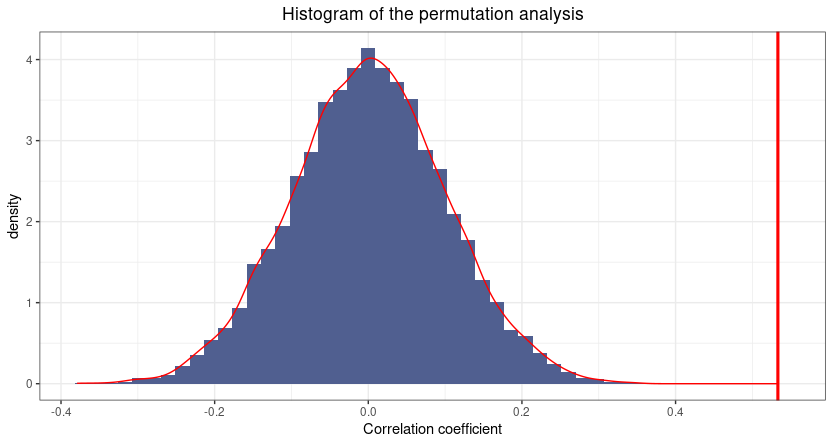
\includegraphics[width=.75\linewidth]{../../week3/data/latex2.png}
          \caption{A subfigure}
          \label{fig:sub2}
        \end{subfigure}
        \label{fig_req}
    \end{figure}

        As seen from \ref{fig:sub1} there is a increase in temperature over time. To verify whether this increase is significant a permutation analysis of the data was done.
        \ref{fig:sub2} shows that the observed correlation is greater than the correlation acquired by random reshuffling. This proves that Florida is getting warmer.

    \end{document}
    